\documentclass{beamer}

\mode<presentation>
{
  \usetheme{Warsaw}
  \setbeamercovered{transparent}
}
\usepackage[english]{babel}
\usepackage[latin1]{inputenc}
\usepackage{times}
\usepackage[T1]{fontenc}

\usepackage{graphicx}
\usepackage{capt-of}
\usepackage{booktabs}
\usepackage{varwidth}

\newcommand{\N}{\mathbb{N}}
\newcommand\Fontvi{\fontsize{8}{8.2}\selectfont}

% Or whatever. Note that the encoding and the font should match. If T1
% does not look nice, try deleting the line with the fontenc.


\title[Dynamic connexity $\&$ parameterised complexity]
{Dynamic connexity $\&$ parameterised complexity}

\subtitle
{Kernelization algorithms: from static to dynamic graphs}

\author[Meyer]
{Pierre~Meyer}

\institute[Universities of Somewhere and Elsewhere]
{
  Department of Computer Science\\
  Ecole Normale Superieure de Lyon}

\date[SL3 2017]
{Soutenance de stage de fin de licence, 2017}

\subject{Theoretical Computer Science}

\pgfdeclareimage[height=0.5cm]{logoENS}{logoENS}
\logo{\pgfuseimage{logoENS}}

% Delete this, if you do not want the table of contents to pop up at
% the beginning of each subsection:
\AtBeginSubsection[]
{
  \begin{frame}<beamer>{Outline}
    \tableofcontents[currentsection,currentsubsection]
  \end{frame}
}

\expandafter\def\expandafter\insertshorttitle\expandafter{%
  \insertshorttitle\hfill%
  \insertframenumber\,/\,\inserttotalframenumber}

\begin{document}

\begin{frame}
  \titlepage
\end{frame}

\begin{frame}{Outline}
  \tableofcontents
  % You might wish to add the option [pausesections]
\end{frame}


\section{Generalising our results}
\subsection{Analysis: Interesting link-stream properties}
\begin{frame}{Graph-Likeness - Time intervals}
  \begin{table}[!h]
    \begin{minipage}{0.4\linewidth}
      \centering
      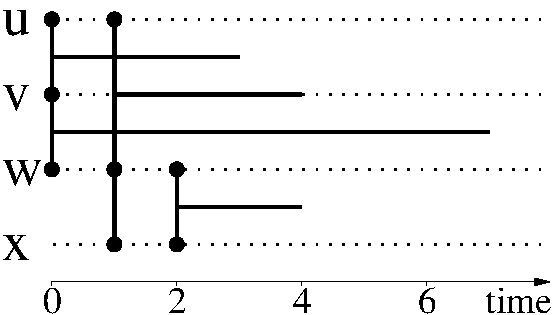
\includegraphics[width=40mm]{exintervals1.pdf}
    \end{minipage}
    \begin{minipage}{0.4\linewidth}
      \centering
      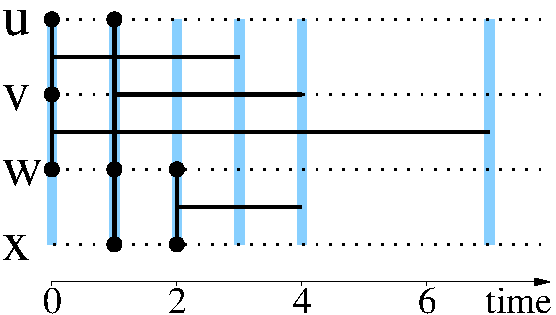
\includegraphics[width=40mm]{exintervals.pdf}
    \end{minipage}
  \end{table}
\end{frame}
\begin{frame}{Neighbourhood Reconstructibility}
  \begin{block}{definition}
    A graph-like class $\Pi$ of link streams is said to be \emph{\bfseries neighbourhood reconstructible} if there are two constants $c,d$ and an algorithm $A$ such that:
    \begin{itemize}
    \item $A$ takes as input a link stream $L$, an integer $k$, and a subset of $V_L$, $V'$, of size not greater than $d$~;
    \item $A$ runs in polynomial time in $size(L)$~;
    \item $A$ decides whether or not $L$ can be transformed, using a total of at most $k$ edition operations and less than $c$ edition operations in the vicinity of any vertex in $V'$, into a link stream $L'\in \Pi$ such that all links of $L'$ have exactly one end in $V'$~.
    \end{itemize}
  \end{block}
\end{frame}
\begin{frame}{Heredity}
  \begin{block}{Definition}
    A class of link streams is said to be \emph{\bfseries hereditary} if it is closed under vertex deletion.
  \end{block}
\end{frame}
\subsection{Synthesis: Similar problems}
\begin{frame}{Problem Denomination: First prefix}
  First prefix: Describes the maximum number of cliques of size $\geq 2$ allowed.
  \begin{itemize}
  \item \emph{\bfseries d-}
  \item \emph{\bfseries *-} (any)
  \end{itemize}
\end{frame}
\begin{frame}{Problem Denomination: Second prefix}
  Second prefix: Describes the maximum number of time intervals.
  \begin{itemize}
  \item \emph{\bfseries If there is no second prefix: } A single time interval, ie: $$\exists b_c, e_c,\ \forall l\in E_L,\ l=(b_c,e_c,\_)$$
  \item \emph{\bfseries -BI-} Two neighbouring intervals, ie: $$\exists (t_{c,i})_{i\in [0,2]},\ \forall l\in E_L,\ \exists i<j,\ l=(t_{c,i},t_{c,j},\_)$$
  \item \emph{\bfseries -MULTI-} Any number of neighbouring intervals $$\exists k,\ \exists (t_{c,i})_{i\in [0,k]},\ \forall l\in E_L,\ \exists i<j,\ l=(t_{c,i},t_{c,j},\_)$$
  \end{itemize}
\end{frame}
\begin{frame}{Problem Denomination: Stem}
  Stem: Describes whether or not we count isolated vertices when counting cliques.
  \begin{itemize}
  \item \emph{\bfseries -Sparse-Split} On each interval, the link stream is a certain number of cliques plus isolated vertices
  \item \emph{\bfseries -Cluster} On each interval, the link stream is a set of disjoint cliques
  \end{itemize}
\end{frame}
\begin{frame}{Problem Classification}
  \begin{minipage}{1\linewidth}
    \centering
    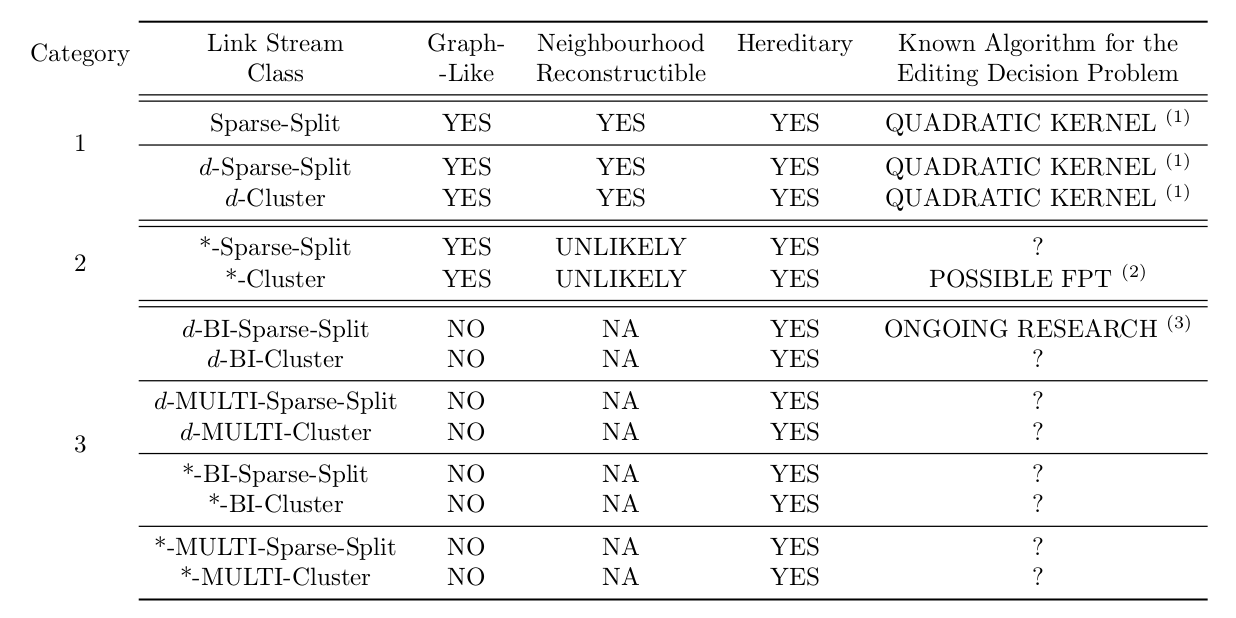
\includegraphics[width=110mm]{perspectives.png}
  \end{minipage}
\end{frame}

\section*{Summary}

\begin{frame}{Summary}
  \begin{itemize}
  \item
    The Sparse-Split Link Stream Editing problem is FPT
  \item
    Many variations thereupon are also FPT
  \end{itemize}
\end{frame}

\end{document}
